
%------------------------------------------------------------------------------------------------------------------
\subsection{TeSSLa passive monitor}\label{subsec:TESLA1}
%\prasad{can this example be written as external monitor? The example can be made into external monitor by separating the execute and terminate scripts of DT and Telegraf+connector+TeSSLA block. The work can be done after the submission but might be manageable. Apologies to Lars/Hannes if the estimation of work required is substantial. Their feedback needs to be taken before making a final decision.}
%\morten{@prasad: Talked to Lars about this. He agreed.}
%This subsection describes the integration of a TeSSLa-based monitoring system as an internal service in the incubator's DT on the DTaaS platform.
%It serves two purposes: reporting on the system status as an external monitor (passive monitor) or directly controlling a part (active monitor). Both options are described in the following subsections.
%\morten{Streamlined subsection/subsubsection structure. Removed intro text (now included in section 4.0)}

As an alternative to NuRV, the RV tool TeSSLa can be utilized for monitoring the DT properties.
Similar to the example presented in~\cite{TT-Connector}, the monitor consists of three parts (see Fig.~\ref{fig:architecture-diagram}).
At its core, the TeSSLa monitor processes input streams and produces output streams, but is not itself capable of integrating them into a larger system context.
A helper function (Connector) is compiled to handle the streams by connecting TeSSLa streams to sockets with which external tools can interact.
Telegraf provides an additional layer of flexibility by adding
\begin{itemize}
	\item reconfigurability at runtime -- the service can be configured to automatically adapt to a changing configuration file using the \lstinline{--watch-config} flag, or simply restarted without losing the internal state of the monitor,
	\item data aggregation with basic statistical operations (such as count, mean, min or histograms),
	\item stream processing for filtering or transforming data streams, and
	\item by providing more than 200 integrations with different services and protocols to send or receive streams\footnote{\url{https://docs.influxdata.com/telegraf/v1/plugins/}}.
\end{itemize}%
%
\begin{figure}[tbp]
	\centering
	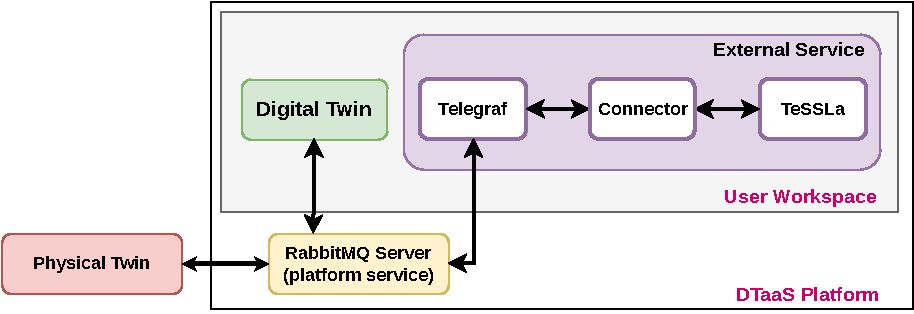
\includegraphics[width=\linewidth]{images/TeSSLa-integration.pdf}
	\caption{Overview of components involved with the TeSSLA passive and active monitors.}
	\label{fig:architecture-diagram}
\end{figure}%
%
The \texttt{create} script prepares the system by ensuring that the necessary tools and software are installed and configured.
It installs Java, Rust and Telegraf on the system, clones the repository for the incubator DT example\footnote{\url{https://github.com/INTO-CPS-Association/example_digital-twin_incubator?tab=readme-ov-file\#running-the-digital-twin}} and downloads the necessary files for the TeSSLa-Telegraf Connector\footnote{\url{https://git.tessla.io/telegraf/tessla-telegraf-connector/-/blob/master/Release/tessla-telegraf-connector.zip}}. Two files, a TeSSLa specification and a Telegraf configuration, must be provided by the user.

A TeSSLa specification suitable for this scenario (shown in Fig.~\ref{fig:tessla_spec_passive}) monitors two key states of the incubator: whether the lid is open and whether the energy saving mode is used, which are passed to the TeSSLa monitor via different event streams.
The helper function \lstinline{raisingDelay} delays any change from \lstinline{false} to \lstinline{true} by three time steps without affecting changes from \lstinline{true} to \lstinline{false}.
This function is used to define an internal data stream \lstinline{critical} that represents when the energy saving mode is expected to be active.
If it is not, an \lstinline{alert} stream is set to \lstinline{true}.
This stream is sent back to the system.
The \lstinline{@TelegrafIn} and \lstinline{@TelegrafOut} annotations allow the compiler to automatically create the Connector function and add to the Telegraf configuration.
%
\begin{figure}[ht]
	\centering
	\begin{lstlisting}
include "./Telegraf.tessla"

@TelegrafIn("amqp_consumer","host=<hostname>", "lid_open")
in lid_open: Events[Bool]

@TelegrafIn("amqp_consumer","host=<hostname>",               "energy_saver_on")
in energy_saver: Events[Bool]

def delayedOpen = raisingDelay(lid_open, 3)
def critical = lid_open && delayedOpen
def alert = critical && !energy_saver

@TelegrafOut("alert")
out alert

def raisingDelay(e: Events[Bool], d: Int): Events[Bool] = merge3(false, const(true, delay(const(d,      boolFilter(e)), e)), const(false, falling(e)))
	\end{lstlisting}
	\caption{a TeSSLa specification for the passive monitor}
	\label{fig:tessla_spec_passive}
\end{figure}%
%
The Telegraf configuration consists of two parts -- where to connect to external data sources and sinks (RabbitMQ in this case), and how to connect to the TeSSLa monitor.
The first has to be specified manually, as it changes from case to case.
Here it configures the AMQP plugin to connect to the RabbitMQ server, subscribe to the topics \lstinline{incubator.diagnosis.plant.lidopen} as well as \lstinline{incubator.energysaver.status} and publish the monitor verdict to the topic \lstinline{incubator.energysaver.alert}.

The \texttt{execute} script uses the following command to add the configuration of how to communicate with the TeSSLa monitor to the supplied Telegraf configuration, create and run the Connector helper function, and compile as well as run the monitor.%
%
\begin{figure}[ht]
	\centering
	\begin{lstlisting}
./TesslaTelegrafConnector -i ./incubator.tessla -c ./telegraf.conf -r
	\end{lstlisting}
	\caption{Command used within execute lifecycle script.}
\end{figure}%

%
The script then starts the Telegraf service with \lstinline{systemctl start telegraf}. This procedure allows data flow to and from the RabbitMQ broker, facilitating the collection, processing and monitoring of sensor data.

The \texttt{terminate} script stops the Telegraf service as well as the TeSSLa monitor and removes all temporary files.

\subsection{TeSSLa active monitor}\label{subsec:TESLA2}
To use TeSSLa as a monitor to directly control the PT, the TeSSLa specification and the Telegraf configuration must be adapted.

To adapt the TeSSLa specification to control the energy saver mode instead of monitoring, the energy saver status is no longer needed as an input and the delayed signal can be provided as an output stream to switch on the energy saver if the lid is still open. As only the rising edge is delayed, the energy saving mode is switched off as soon as the lid is closed again.

The notable change in the Telegraf configuration is the line shown in Fig.~\ref{fig:telegraf_json_transformation} in the AMQP output plugin, which translates the boolean value for controlling the energy saving mode into the JSON format required by the incubator. It uses the JSONata\footnote{\url{https://jsonata.org/}} transformation style.
By adding this post-processing step to Telegraf\footnote{
	Telegraf first introduced the JSON transformation feature in version 1.24, which has not yet been widely distributed to package repositories.
}, the user is able to change the formatting or desired temperature setting in the running system by changing the configuration without recompiling the monitor or losing its internal state.%
%
\begin{figure}[H]
	\begin{lstlisting}
transform = '{"temperature_desired": fields.value ? 21 : 35}'
    \end{lstlisting}
	\caption{Telegraf JSON transformation}
	\label{fig:telegraf_json_transformation}
\end{figure}















% notes for reference only –– TeSSLa spec for active mode and Telegraf conf
\iffalse



	% telegraf passive – shordened
	\begin{figure}[ht]
		\centering
		\begin{lstlisting}[style=code]
\begin{lstlisting}[style=code]
[agent]
interval = "1s"
flush_interval = "1s"
[[inputs.amqp_consumer]]
    <...>
	binding_key = "incubator.diagnosis.plant.lidopen"
	json_string_fields = ["lid_open"]
[[inputs.amqp_consumer]]
    <...>
	binding_key = "incubator.energysaver.status"
	json_string_fields = ["energy_saver_on"]
[[outputs.amqp]]
    <...>
	routing_key = "incubator.energysaver.alert"

[[outputs.socket_writer]]
  urls = ["udp://localhost:1653"]
  data_format = "influx"
[[inputs.socket_listener]]
  service_address = "udp://localhost:1654"
  data_format = "influx"
	\end{lstlisting}
		\caption{Telegraf configuration for the TeSSLa Monitor. Some fields have been dropped for brevity. See \lars{link to repository} for the complete configuration. \lars{ToDo: remove + link and explain in text}}
	\end{figure}


	% telegraf passive
	\begin{figure}[ht]
		\centering
		\begin{lstlisting}[style=code]

[agent]
interval = "1s"
flush_interval = "1s"
[[inputs.amqp_consumer]]
	brokers = ["amqp://localhost:5672"]
	username = "incubator"
	password = "incubator"
	exchange = "Incubator_AMQP"
	exchange_durability = "transient"
 	data_format = "json"
  	queue = "telegraf"
	queue_durability = "transient"
	binding_key = "incubator.diagnosis.plant.lidopen"
	json_string_fields = ["lid_open"]

[[inputs.amqp_consumer]]
    <...>
  	queue = "telegraf"
	queue_durability = "transient"
	binding_key = "incubator.energysaver.status"
	json_string_fields = ["energy_saver_on"]

[[outputs.amqp]]
    <...>
	routing_key = "incubator.energysaver.alert"
	namepass = ["alert"]

[[outputs.file]]
	files = ["stdout"]

[[outputs.influxdb]]
  urls = ["udp://localhost:1653"]

[[inputs.socket_listener]]
  service_address = "udp://localhost:1654"
  data_format = "influx"
	\end{lstlisting}
		\caption{Telegraf configuration for the TeSSLa Monitor. The redundant fields of the second AMQP consumer have been dropped for brevity.\lars{move to appendix or provide link to repository?}}
	\end{figure}

	\begin{figure}[H]
		\centering
		\begin{lstlisting}[style=code]
include "./Telegraf.tessla"

@TelegrafIn("amqp_consumer","host=<hostname>", "lid_open")
in lid_open: Events[Bool]

def delayedOpen = raisingDelay(lid_open, 3)
def result = lid_open && delayedOpen

@TelegrafOut("result")
out result
def raisingDelay(e: Events[Bool], d: Int): Events[Bool] = merge3(false, const(true, delay(const(d, boolFilter(e)), e)), const(false, falling(e)))
	\end{lstlisting}
		\caption{TeSSLa specification}
		\label{fig:tessla_spec_active}
	\end{figure}



	\begin{figure}[ht]
		\centering
		\begin{lstlisting}[style=code]
[agent]
interval = "1s"
flush_interval = "1s"

[[inputs.amqp_consumer]]
	brokers = ["amqp://localhost:5672"]
	username = "incubator"
	password = "incubator"
	exchange = "Incubator_AMQP"
	exchange_durability = "transient"
	queue = "telegraf"
	queue_durability = "transient"
	binding_key = "incubator.diagnosis.plant.lidopen"
	data_format = "json"
	json_string_fields = ["lid_open"]

[[inputs.amqp_consumer]]
	brokers = ["amqp://localhost:5672"]
	username = "incubator"
	password = "incubator"
	exchange = "Incubator_AMQP"
	exchange_durability = "transient"
	queue = "telegraf"
	queue_durability = "transient"
	binding_key = "incubator.energysaver.status"
	data_format = "json"
	json_string_fields = ["energy_saver_on"]

[[outputs.amqp]]
	brokers = ["amqp://localhost:5672"]
	username = "incubator"
	password = "incubator"
	exchange = "Incubator_AMQP"
	exchange_durability = "transient"
	routing_key = "incubator.update.closed_loop_controller.parameters"
	namepass = ["result"]
	data_format = "json"
	use_batch_format = false
    json_transformation = '{"temperature_desired" : fields.value ? 21 : 35}'


[[outputs.file]]
	files = ["stdout"]


[[outputs.influxdb]]
  urls = ["udp://127.0.0.1:1653"]
[[inputs.socket_listener]]
  service_address = "udp://:1654"
  data_format = "influx"
	\end{lstlisting}
		\caption{Telegraf configuration for the TeSSLa Monitor. The redundant fields of the second AMQP consumer have been dropped for brevity.}
		\label{fig:telegraf_conf}
	\end{figure}

\fi


%------------------------------------------------------------------------------------------------------------------
